\documentclass{article}

\usepackage{amsmath, amssymb}
\usepackage[margin=0.7in]{geometry}
\usepackage{float}
\usepackage{graphicx}
\usepackage{epstopdf}
\restylefloat{table}

\author{Guillaume Labranche (260585371)}
\title{Assignment \#4\\Numerical Computing (COMP 350)}
\date{due on 2 November 2015}

\newcommand{\R}{\mathbb{R}}
\newcommand{\F}{\mathbb{F}}

\begin{document}

\maketitle
 
\begin{enumerate}
\item \begin{enumerate}
\item 
\item We start with the Taylor series expansion of $f(x)$ about $x_0$:
\begin{align*}
f(x) &= f(x_0) + f'(x_0)(x-x_0) + \frac{f''(x_0)}{2}(x-x_0)^2 \\
f(x) &= f(x_0) + \Big(f'(x_0) + \frac{f''(x_0)}{2}(x-x_0)\Big) (x-x_0)
\end{align*}
We use the facts that $f(x)=0$ and $(x-x_0)=-\frac{f(x_0)}{f'(x_0)}$ (Newton's method):
\begin{align*}
0 &= f(x_0) + \Big(f'(x_0) - \frac{f''(x_0)}{2} \cdot \frac{f(x_0)}{f'(x_0)} \Big) (x-x_0) \\
x-x_0 &= \frac{-f(x_0)}{f'(x_0) - \frac{f''(x_0) f(x_0)}{2 f'(x_0)}} \\
x &= x_0 - \frac{2f(x_0)f'(x_0)}{2\big[f'(x_0)\big]^2 - f(x_0) f''(x_0)} 
\end{align*}
This is also known as Halley's method. See attached file \texttt{halley.m} for its implementation.
\end{enumerate}
\item The computed roots for each methods are in Table \ref{table:roots} and the results of each of their iteration steps are in Tables \ref{table:bisection}, \ref{table:newton}, \ref{table:halley} and \ref{table:secant}. The graph of $y=f(x)$ (in green) and $y=f'(x)$ (in red) are in Figure \ref{fig:q2plot}.

See attached function files \texttt{halley.m} and \texttt{secant.m} for the implementation of the new root-finding methods.

See attached function files \texttt{f.m}, \texttt{fd.m} and \texttt{fdd.m} for the implementation of $f(x)$, $f'(x)$ and $f''(x)$.

See attached script file \texttt{q2.m} for the commands generating the results and the plot. In this case, we used $n_{max}=10^5$, $x_0=1$, $x_1=2$.

As we can see, Halley's method is the fastest with 3 iterations since it has cubic convergence but it requires $f'(x)$ and $f''(x)$. Newton's method comes as a close second with 4 iterations since it converges quadratically but requires $f'(x)$. Not far after, the secant method converging super-linearly takes 8 iterations to reach the same degree of precision without requiring a derivative of $f(x)$. Then far behind the others, the bisection method took 40 iterations. That is 5 times more than the next fastest method and more than 13 times more than the fastest, because it has linear convergence.

\begin{table}[h]
  \centering
  \begin{tabular}{| l | l | c |}
  \hline
  Method & Computed root & Number of iterations\\ \hline
  Bisection & $1.834243184314801$ & $40$ \\ \hline
  Newton's & $1.834243184314032$ & $4$ \\ \hline
  Halley's & $1.834243184313922$ & $3$ \\ \hline
  Secant & $1.834243184313922$ & $8$ \\ \hline
  \end{tabular}
  \caption{Comparison of all methods}
  \label{table:roots}
\end{table}

\begin{table}[h]
  \centering
  \footnotesize
\begin{tabular}{| r | r | r | r | r |}
\hline
$a$ & $b$ & $c$ & $f(c)$ & error\_bound\\
\hline
$  1.000000000000000e+00$ & $  2.000000000000000e+00$ & $  1.500000000000000e+00$ & $ -1.125000000000000e+00$ & $  5.000000000000000e-01$\\
$  1.500000000000000e+00$ & $  2.000000000000000e+00$ & $  1.750000000000000e+00$ & $ -3.906250000000000e-01$ & $  2.500000000000000e-01$\\
$  1.750000000000000e+00$ & $  2.000000000000000e+00$ & $  1.875000000000000e+00$ & $  2.167968750000000e-01$ & $  1.250000000000000e-01$\\
$  1.750000000000000e+00$ & $  1.875000000000000e+00$ & $  1.812500000000000e+00$ & $ -1.081542968750000e-01$ & $  6.250000000000000e-02$\\
$  1.812500000000000e+00$ & $  1.875000000000000e+00$ & $  1.843750000000000e+00$ & $  4.891967773437500e-02$ & $  3.125000000000000e-02$\\
$  1.812500000000000e+00$ & $  1.843750000000000e+00$ & $  1.828125000000000e+00$ & $ -3.095626831054688e-02$ & $  1.562500000000000e-02$\\
$  1.828125000000000e+00$ & $  1.843750000000000e+00$ & $  1.835937500000000e+00$ & $  8.645534515380859e-03$ & $  7.812500000000000e-03$\\
$  1.828125000000000e+00$ & $  1.835937500000000e+00$ & $  1.832031250000000e+00$ & $ -1.123923063278198e-02$ & $  3.906250000000000e-03$\\
$  1.832031250000000e+00$ & $  1.835937500000000e+00$ & $  1.833984375000000e+00$ & $ -1.317836344242096e-03$ & $  1.953125000000000e-03$\\
$  1.833984375000000e+00$ & $  1.835937500000000e+00$ & $  1.834960937500000e+00$ & $  3.658599220216274e-03$ & $  9.765625000000000e-04$\\
$  1.833984375000000e+00$ & $  1.834960937500000e+00$ & $  1.834472656250000e+00$ & $  1.169069320894778e-03$ & $  4.882812500000000e-04$\\
$  1.833984375000000e+00$ & $  1.834472656250000e+00$ & $  1.834228515625000e+00$ & $ -7.471149729099125e-05$ & $  2.441406250000000e-04$\\
$  1.834228515625000e+00$ & $  1.834472656250000e+00$ & $  1.834350585937500e+00$ & $  5.470969099405920e-04$ & $  1.220703125000000e-04$\\
$  1.834228515625000e+00$ & $  1.834350585937500e+00$ & $  1.834289550781250e+00$ & $  2.361722065415961e-04$ & $  6.103515625000000e-05$\\
$  1.834228515625000e+00$ & $  1.834289550781250e+00$ & $  1.834259033203125e+00$ & $  8.072522976476648e-05$ & $  3.051757812500000e-05$\\
$  1.834228515625000e+00$ & $  1.834259033203125e+00$ & $  1.834243774414063e+00$ & $  3.005585032411773e-06$ & $  1.525878906250000e-05$\\
$  1.834228515625000e+00$ & $  1.834243774414063e+00$ & $  1.834236145019531e+00$ & $ -3.585327642952052e-05$ & $  7.629394531250000e-06$\\
$  1.834236145019531e+00$ & $  1.834243774414063e+00$ & $  1.834239959716797e+00$ & $ -1.642392577316798e-05$ & $  3.814697265625000e-06$\\
$  1.834239959716797e+00$ & $  1.834243774414063e+00$ & $  1.834241867065430e+00$ & $ -6.709190389031505e-06$ & $  1.907348632812500e-06$\\
$  1.834241867065430e+00$ & $  1.834243774414063e+00$ & $  1.834242820739746e+00$ & $ -1.851807683195261e-06$ & $  9.536743164062500e-07$\\
$  1.834242820739746e+00$ & $  1.834243774414063e+00$ & $  1.834243297576904e+00$ & $  5.768874231648624e-07$ & $  4.768371582031250e-07$\\
$  1.834242820739746e+00$ & $  1.834243297576904e+00$ & $  1.834243059158325e+00$ & $ -6.374604426540032e-07$ & $  2.384185791015625e-07$\\
$  1.834243059158325e+00$ & $  1.834243297576904e+00$ & $  1.834243178367615e+00$ & $ -3.028658746018209e-08$ & $  1.192092895507813e-07$\\
$  1.834243178367615e+00$ & $  1.834243297576904e+00$ & $  1.834243237972260e+00$ & $  2.733003983124149e-07$ & $  5.960464477539063e-08$\\
$  1.834243178367615e+00$ & $  1.834243237972260e+00$ & $  1.834243208169937e+00$ & $  1.215069005411351e-07$ & $  2.980232238769531e-08$\\
$  1.834243178367615e+00$ & $  1.834243208169937e+00$ & $  1.834243193268776e+00$ & $  4.561015476411967e-08$ & $  1.490116119384766e-08$\\
$  1.834243178367615e+00$ & $  1.834243193268776e+00$ & $  1.834243185818195e+00$ & $  7.661783207879580e-09$ & $  7.450580596923828e-09$\\
$  1.834243178367615e+00$ & $  1.834243185818195e+00$ & $  1.834243182092905e+00$ & $ -1.131240257024047e-08$ & $  3.725290298461914e-09$\\
$  1.834243182092905e+00$ & $  1.834243185818195e+00$ & $  1.834243183955550e+00$ & $ -1.825309681180443e-09$ & $  1.862645149230957e-09$\\
$  1.834243183955550e+00$ & $  1.834243185818195e+00$ & $  1.834243184886873e+00$ & $  2.918237207438779e-09$ & $  9.313225746154785e-10$\\
$  1.834243183955550e+00$ & $  1.834243184886873e+00$ & $  1.834243184421212e+00$ & $  5.464642072183779e-10$ & $  4.656612873077393e-10$\\
$  1.834243183955550e+00$ & $  1.834243184421212e+00$ & $  1.834243184188381e+00$ & $ -6.394227369810324e-10$ & $  2.328306436538696e-10$\\
$  1.834243184188381e+00$ & $  1.834243184421212e+00$ & $  1.834243184304796e+00$ & $ -4.648015305974695e-11$ & $  1.164153218269348e-10$\\
$  1.834243184304796e+00$ & $  1.834243184421212e+00$ & $  1.834243184363004e+00$ & $  2.499920270793155e-10$ & $  5.820766091346741e-11$\\
$  1.834243184304796e+00$ & $  1.834243184363004e+00$ & $  1.834243184333900e+00$ & $  1.017559370097843e-10$ & $  2.910383045673370e-11$\\
$  1.834243184304796e+00$ & $  1.834243184333900e+00$ & $  1.834243184319348e+00$ & $  2.763833606422850e-11$ & $  1.455191522836685e-11$\\
$  1.834243184304796e+00$ & $  1.834243184319348e+00$ & $  1.834243184312072e+00$ & $ -9.420908497759228e-12$ & $  7.275957614183426e-12$\\
$  1.834243184312072e+00$ & $  1.834243184319348e+00$ & $  1.834243184315710e+00$ & $  9.109157872444484e-12$ & $  3.637978807091713e-12$\\
$  1.834243184312072e+00$ & $  1.834243184315710e+00$ & $  1.834243184313891e+00$ & $ -1.563194018672220e-13$ & $  1.818989403545857e-12$\\
$  1.834243184313891e+00$ & $  1.834243184315710e+00$ & $  1.834243184314801e+00$ & $  4.476419235288631e-12$ & $  9.094947017729282e-13$\\
\hline
\end{tabular}

  \caption{Results of the bisection method}
  \label{table:bisection}
\end{table}

\begin{figure}
  \centering
  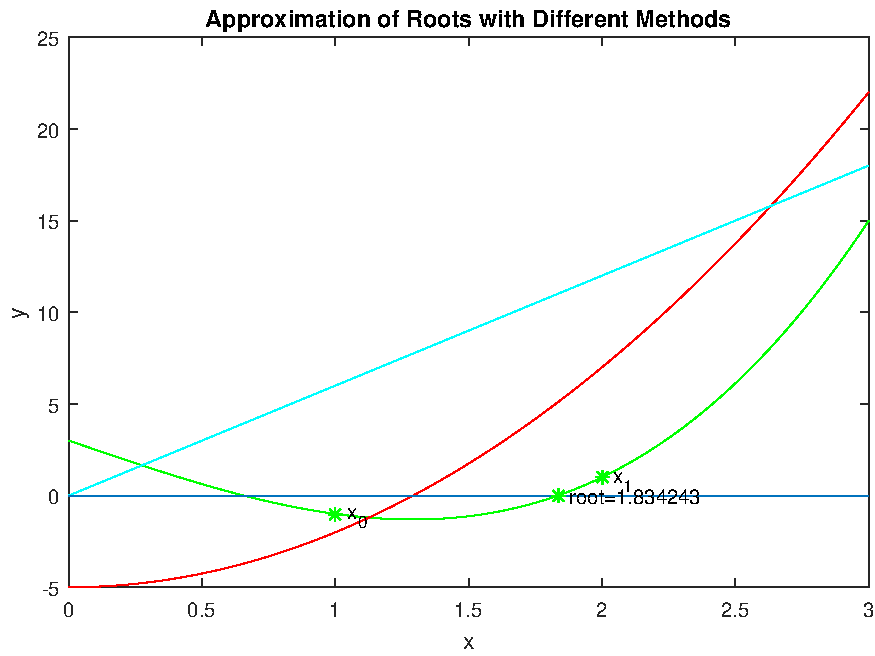
\includegraphics[width=0.8\textwidth]{q2plotv}
  \caption{$f(x)$ is shown in green, with the points $\big(x_0,f(x_0)\big)$ and $\big(x_1,f(x_1)\big)$. $f'(x)$ and $f''(x)$ are shown in red and cyan.}
  \label{fig:q2plot}
\end{figure}

\begin{table}[h]
  \centering
  \begin{tabular}{| r | r | r |}
\hline
$n$ & $x$ & $f(x)$\\
\hline
$   0$ & $  2.000000000000000e+00$ & $  1.000000000000000e+00$\\
$   1$ & $  1.857142857142857e+00$ & $  1.195335276967926e-01$\\
$   2$ & $  1.834787350054526e+00$ & $  2.773253015902810e-03$\\
$   3$ & $  1.834243503918507e+00$ & $  1.627856713426468e-06$\\
$   4$ & $  1.834243184314032e+00$ & $  5.622169396701793e-13$\\
\hline
\end{tabular}

  \caption{Results of the Newton's method}
  \label{table:newton}
\end{table}

\begin{table}[h]
  \centering
  \begin{tabular}{| r | r | r | r | r |}
\hline
$n$ & $x$ & $f(x)$ & $f'(x)$ & $f''(x)$\\
\hline
$   0$ & $  2.000000000000000e+00$ & $  1.000000000000000e+00$ & $  7.000000000000000e+00$ & $  1.200000000000000e+01$\\
$   1$ & $  1.837209302325581e+00$ & $  1.515589822279662e-02$ & $  5.126014061654949e+00$ & $  1.102325581395349e+01$\\
$   2$ & $  1.834243209456139e+00$ & $  1.280579668971882e-07$ & $  5.093344454307868e+00$ & $  1.100545925673683e+01$\\
$   3$ & $  1.834243184313922e+00$ & $  8.881784197001252e-16$ & $  5.093344177606227e+00$ & $  1.100545910588353e+01$\\
\hline
\end{tabular}

  \caption{Results of Halley's method}
  \label{table:halley}
\end{table}

\begin{table}[h]
  \centering
  \begin{tabular}{| r | r | r |}
\hline
$n$ & $x_1$ & $f(x_1)$\\
\hline
$   0$ & $  2.000000000000000e+00$ & $  1.000000000000000e+00$\\
$   1$ & $  1.500000000000000e+00$ & $ -1.125000000000000e+00$\\
$   2$ & $  1.764705882352941e+00$ & $ -3.279055566863436e-01$\\
$   3$ & $  1.873599540361965e+00$ & $  2.090397299390610e-01$\\
$   4$ & $  1.831205833909406e+00$ & $ -1.541953360163717e-02$\\
$   5$ & $  1.834118127083818e+00$ & $ -6.368734578741098e-04$\\
$   6$ & $  1.834243595856441e+00$ & $  2.096128623563232e-06$\\
$   7$ & $  1.834243184258313e+00$ & $ -2.832365453286911e-10$\\
$   8$ & $  1.834243184313922e+00$ & $ -1.776356839400251e-15$\\
\hline
\end{tabular}

  \caption{Results of the secant method}
  \label{table:secant}
\end{table}
\end{enumerate}
\end{document}